%-----------------------------------------------------------------------------80
% SECTION TITLE|
%-----------------------------------------------------------------------------80

\section{Modificadores de formato}  

%-----------------------------------------------------------------------------80
% CONTENT
%-----------------------------------------------------------------------------80

\subsection{Formatos de representación de datos}

\begin{frame}[fragile]{Modificadores de formato} 
    \begin{itemize}[<+(1)->]
        \item Existen dos tipos de datos: formatedos y no formateados.
        \item Los datos formateados son aquellos representados por caracteres de texto, es decir, cadenas de caracteres.
        \item Los datos no formateados son aquellos represntados por código binario o código máquina.
        \item En el caso de los formateados tenemos los automáticos y los preestablecidos.
    \end{itemize}
\end{frame}

\begin{frame}[fragile]{Formatos de representación de datos} 
  \textbf{Formatos automáticos}
    \begin{itemize}[<+(1)->] 
        \item Se da a partir del uso del "*" en \emph{read}, \emph{print} y \emph{write}.
          \vspace{0.1cm}
        \item []
            \begin{minted}[linenos,autogobble]{fortran}
                print* <expresion1>, ...
                read* <expresion1>, ...
                write(*,*) <expresion1>, ...
                read(*,*) <expresion1>, ...
                write(6,*) <expresion1>, ...
                read(5,*) <expresion1>, ...
            \end{minted}
        \item En el uso de \emph{read}, los datos deben estar separados por espacios o comas. Los tipo character, delimitados por comillas simples/dobles.
        \item Para la escritura de datos, el procesador proporcionará: \\ 
        - datos tipo numérico de manera completa según se especifique. \\ 
        - datos tipo \emph{logical} utilizando los caracteres T y F (.true. .false.).\\
        - datos tipo \emph{character} de acuerdo a la longitud de la expresión.
    \end{itemize}
\end{frame}

\begin{frame}[fragile]{Formatos de representación de datos} 
  \textbf{Formatos preestablecidos}
    \begin{itemize}[<+(1)->] 
        \item Estos tipos de formatos permiten facilitar la creación de arreglos y reutilizar datos obtenidos.
        \item [] \textbf{Especificadores de Campo y Formato}
        \item La unidad de registro de lectura y escritura es la línea de texto. Está subdividida en celdas y cada una alberga un caracter.
        \item Cada celda puede ser parte de un campo, en donde se especifique cierto formato.
        \vspace{0.1cm}
        \item []
            \begin{figure}
                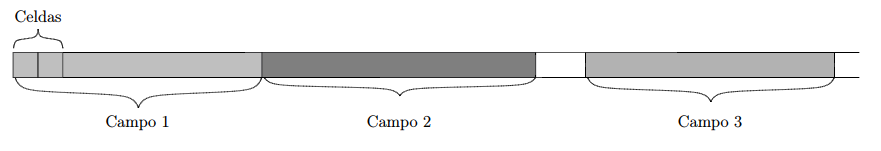
\includegraphics[width=0.8\textwidth]{./resources/specifiers.png}
                \caption*{Campos de escritura y lectura en una Línea de texto}
            \end{figure}
        \item Los especificadores más relevantes se explicarán a continuación:
    \end{itemize}
\end{frame}

\begin{frame}[fragile]{Formatos de representación de datos} 
  \textbf{Especificador de tipo Integer I\textit{n}}
    \begin{itemize}[<+(1)->] 
        \item El valor es representado en notación usual decimal.
        \item Si el valor es negativo, el signo - irá a la izquierda del primer dígito sin espacio de separación.
        \item Si se utilizan varios dígitos, estos ván juntos, sin espacios de separación y el primer dígito a la izquierda es diferente de 0.
        \item El dígito correspondiente a las unidades está ubicado en el extremo derecho de la cadena de caracteres utilizada.
        \item Los caracteres a la izquierda del primer dígito o eventualmente el signo - son espacios.
    \end{itemize}
\end{frame}

\begin{frame}[fragile]{Formatos de representación de datos} 
  \textbf{Especificador punto fijo de tipo Real F\textit{n.d}}
    \begin{itemize}[<+(1)->] 
        \item El valor es representado en notación usual decimal.
        \item En caso que el número sea negativo, el caracter - va a la izquierda de la parte entera o el punto (si la parte entera es 0), sin espacios.
        \item La parte fraccionaria del valor real ocupa los últimos $d$ caracteres del campo sin espacios, solamente dígitos (0-9), el caracter anterior a la parte fraccionaria corresponde al caracter punto “.”.
        \item Los dígitos de la parte entera del valor van a la izquierda del punto, sin espacios de separación. En caso que la parte entera sea diferente de 0, el primer dígito es diferente de 0; en el caso que la parte entera sea 0, el primer dígito es 0 o ningún caracter.
    \end{itemize}
\end{frame}

\begin{frame}[fragile]{Formatos de representación de datos} 
  \textbf{Especificador punto flotante de tipo Real (simple presición) E\textit{n.d}}
    \begin{itemize}[<+(1)->] 
        \item Las últimas cuatro plazas del campo están reservadas para el exponente, comienza con la letra E, seguido del signo + o del signo - y dos dígitos (0-9); es decir, por ejemplo E+09.
        \item La parte fraccionaria de la representación en punto flotante del valor real ocupan los $d$ caracteres del campo antes de la parte asignada al exponente sin espacios. Los caracteres asignados para la parte fraccionaria son únicamente dígitos (0-9).
        \item El caracter “.” va a la izquierda de la parte decimal, sin espacios.
        \item La parte entera está representada por 0 o níngun caracter y va a la izquierda del punto, sin espacios de separación.
        \item En caso que el número sea negativo, el caracter - va a la izquierda de la parte entera o el punto sin espacios.
        \item El \textbf{especificador punto flotante de tipo Real (doble presición) D\textit{n.d}} obedece a las anteriores reglas.
    \end{itemize}
\end{frame}

\begin{frame}[fragile]{Formatos de representación de datos} 
  \textbf{Especificador punto de tipo character A y A\textit{d}}
    \begin{itemize}[<+(1)->] 
        \item Se emplean para expresiones que pueden tomar distintos valores.
        \item En la escritura se puede asignar una cadena de caracteres de cierta longitud mediante '=' y entre comillas.
    \end{itemize}
 \onslide<4-> \textbf{Especificador punto de tipo logical L y L\textit{d}}
    \begin{itemize}[<+(2)->] 
        \item El especificador L utiliza un campo de dos caracteres mientras L\textit{d} uno para \textit{d} caracteres.
    \end{itemize}
\end{frame}

\begin{frame}[fragile]{Modificadores de formato}
   \begin{table}[]
    \centering
    \label{Tabla_especificaciones}
    \resizebox{10.55cm}{!} {
      \begin{tabular}{|l|l|l|}
        \hline
        \textbf{Esp.}   & \textbf{Nombre}                   & \textbf{Acción}                                                               \\ \hline    
        I\textit{n}     & Entero                            & Asigna un campo de $n$ caracteres para representar un entero en notación      \\          
                        &                                   & decimal, justificado por derecha.                                             \\ \hline
        F\textit{n.d}   & Punto fijo                        & Asigna un campo de $n$ caracteres para representar un real en formato punto   \\    
                        &                                   & fijo, con $d$ dígitos para la parte fraccionaria, justificado por la derecha. \\ \hline
        E\textit{n.d}   & Punto flotante                    & Asigna un campo de $n$ caracteres para representar un real en formato punto   \\  
                        &                                   & flotante, con $d$ dígitos para la parte fraccionaria, justificado por derecha.\\ \hline  
        D\textit{n.d}   & Punto flotante doble presición    & Lo mismo que especificador E, pero en doble presición.                        \\ \hline
        g\textit{n.d}   & Real                              & Asigna una campo de longitud $n$, con $d$ dígitos; dependiendo del valor:     \\     
                        &                                   & en punto fijo, justificación a la la izquierda o punto flotante,              \\
                        &                                   & justificación a la derecha.                                                   \\ \hline
        A\textit{n}     & Texto                             & Asigna un campo de longitud $n$, para expresiones de tipo $character$.        \\ \hline
        A               & Texto                             & Asigna un campo de longitud, la longitud de la expresión de tipo $character$. \\ \hline
        $\ldots$        & Texto fijo                        & Asigna el campo de longitud la cadena de caracteres y escribe en el campo .   \\
                        &                                   & la cadena.                                                                    \\ \hline
        L\textit{n}     & Lógico                            & Asigna un campo de $n$ caracteres para valores lógicos, justificación a       \\ 
                        &                                   & la derecha.                                                                   \\ \hline
        L               & Lógico                            & Asigna un campo de dos caracteres para valores lógicos, justificación por     \\ \hline 
                        &                                   & la derecha.                                                                   \\ \hline 
        X               & Espacio                           & Desplaza el siguiente campo de un espacio.                                    \\ \hline
        T\textit{n}     & Tabulador                         & El siguiente campo comienza en la columna $n$.                                \\ \hline
        \$              & Manteción de la línea             & No cambia la linea al final una instrucción de escritura o lectura.           \\ \hline
        /               & Cambio de línea                   & Cambia de línea.                                                              \\ \hline
      \end{tabular}}
          \caption*{Principales especificadores de formato y control}          
    \end{table}
\end{frame}


